% 这个文件存在的目的是为了帮助我自己学习tikz。
\documentclass{article}
\usepackage{tikz}
\usetikzlibrary{intersections} %专门为交点的使用而创建,请看后面
\begin{document}
now we begin!
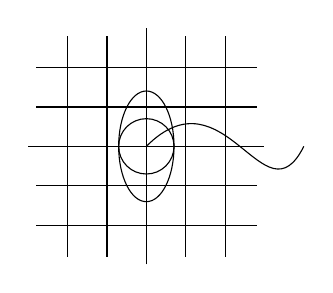
\begin{tikzpicture}


  % 设置线条的style
  % 使用方法是:
  % help lines是给这种style起的名字,后面的大括号里是进行的设置
  % 可以换名字,也可以在大括号里增添内容;
  % 当你要使用这个style时,你只需要在那个draw的后面添加上[你定义的style
  % 的名字]即可。

  liangzi grid/.style={color=blue!50,very thin}

  help lines/.style={color=blue!100}

  
  % 画直线
  \draw (-1.5,0) -- (1.5,0);
  \draw (0,-1.5) -- (0,1.5);

  % 画曲线
  \draw (0,0) .. controls (1,1) and (1.5, -1) .. (2,0);

  % 画圆和椭圆
  \draw (0,0) circle [radius=10pt];
  \draw (0,0) ellipse [x radius=10pt, y radius=20pt];

  % 长方形
  \draw (0,0) rectangle (1,1);

  % 网格线
  % step是设置每条网格线之间的间隔的数值。
  % grid前面的参数是设置网格线的起点横坐标和纵坐标,而右侧是重点。
  \draw[step=.5cm] (-1.4,-1.4) grid (1.4,1.4);

\end{tikzpicture}


\begin{tikzpicture}[scale=3]  % scale=3 就是放大三倍的意思
  
  % 剪切一个矩阵,其大小是从(-0.1,-0.2)to (1.1,0.75)
  \clip (-1.6,-1.7) rectangle (2,2);

  % 绘制网格线,之前提到过
  \draw[step=.5cm,gray,very thin] (-1.4,-1.4) grid (1.4,1.4);

  % 画直线,不再解释
  % -> 代表箭头,正方向的
  \draw [->] (-1.5,0) -- (1.5,0);

  % <- 反方向
  \draw [<-] (0,-1.5) -- (0,1.5);

  \draw (0,0) circle [radius=1cm];

  % fill+draw,就是右填充又描边的意思.其中,[]写的是颜色的配置,
  % green!20!back指的是20%的绿混合80%的黑
  \filldraw[fill=green!20,draw=green!50!black] (0,0) -- (3mm,0mm)

  % arc专门用于画弧线。起始角度、终止角度、半径都被提及了
  arc [start angle=0, end angle=30, radius=3mm] -- cycle;


  % very thick 就是很厚的意思。
  % + 用于相对坐标系,表示在之前点(亦即极坐标(30:1cm)的基础上向下移动
  % 0.5cm得到的点。--表示将这两个点拼接)
  %
  \draw[red,very thick] (30:1cm) -- +(0,-0.5);

  \draw[blue,very thick] (30:1cm) ++(0,-0.5) -- (0,0);

\end{tikzpicture}


% 下面这两个例子是对比+ 与++的区别的。但是我真的没有看出来他们有什么区别。
\begin{tikzpicture}
\def\rectanglepath{-- ++(1cm,0cm) -- ++(0cm,1cm) -- ++(-1cm,0cm) -- cycle}
\draw (0,0) \rectanglepath;
\draw (10,0) \rectanglepath;
\end{tikzpicture}


\begin{tikzpicture}
\def\rectanglepath{-- +(1cm,0cm) -- +(1cm,1cm) -- +(0cm,1cm) -- cycle}
\draw (0,0) \rectanglepath;
\draw (10,0) \rectanglepath;
\end{tikzpicture}

% 同样地,他们可以被下面这行程序替代

\tikz \draw (0,0) rectangle +(1,1) (10,0) rectangle +(1,1);

% 演示如何获取两条线的交点
\begin{tikzpicture}
% 定义一条直线,名字是ypward line   
\path [name path=upward line] (1,0) -- (1,1);

\path [name path=sloped line] (0,0) -- (30:1.5cm); % a bit longer, so that there is an intersection
% (add `\usetikzlibrary{intersections}' after loading tikz in the preamble)
% intersections 操作就是为了获取交点。of STH and STH,命名为STH.
% 之后就是利用这个名为x的点。
\draw [name intersections={of=upward line and sloped line, by=x}]
[very thick,orange] (1,0) -- (x);
\end{tikzpicture}


% 通过箭头画图的一个示意
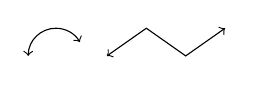
\begin{tikzpicture}
\draw [<->] (0,0) arc [start angle=180, end angle=30, radius=10pt];
\draw [<->] (1,0) -- (1.5cm,10pt) -- (2cm,0pt) -- (2.5cm,10pt);
\end{tikzpicture}

\usetikzlibrary {arrows.meta}
\begin{tikzpicture}[>=Stealth] % 可能是代表尖箭头的意思吧
\draw [->] (0,0) arc [start angle=180, end angle=30, radius=10pt];
\draw [<<-,very thick] (1,0) -- (1.5cm,10pt) -- (2cm,0pt) --
(2.5cm,10pt);    % 双箭头
\end{tikzpicture}

% 这个示例主要展示了如何使用scope进行局部地区屏蔽并自定义格式的功能。
\begin{tikzpicture}[ultra thick]
\draw (0,0) -- (0,1);
\begin{scope}[thin]
\draw (1,0) -- (1,1);
\draw (2,0) -- (2,1);
\end{scope}
\draw (3,0) -- (3,1);
\end{tikzpicture}

% 这个示例主要展示坐标系移动的命令
% 可以看出,下面的命令让x轴向左移动了2pt?
\tikz \draw (0,0) -- (0,0.5) [xshift=2pt] (0,0) -- (0,1);


% 下图显示了平移旋转等的transformation。
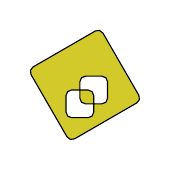
\begin{tikzpicture}[even odd rule,rounded corners=2pt,x=10pt,y=10pt]
\filldraw[fill=yellow!80!black] (0,0) rectangle (1,1)
[xshift=5pt,yshift=5pt] (0,0) rectangle (1,1)
[rotate=30] (-1,-1) rectangle (2,2);
\end{tikzpicture}

% 用循环的方式画圆,其中...可以省略中间的东西
\tikz \foreach \x in {1,...,10}
\draw (\x,0) circle (0.4cm);

% 插入文字.
% 使用的是node命令。
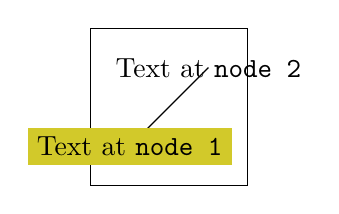
\begin{tikzpicture}
\draw (0,0) rectangle (2,2);
\draw (0.5,0.5) node [fill=yellow!80!black]
{Text at \verb!node 1!}
-- (1.5,1.5) node {Text at \verb!node 2!};
\end{tikzpicture}


% 这个示例是在展示把node的位置放置在哪里的问题。
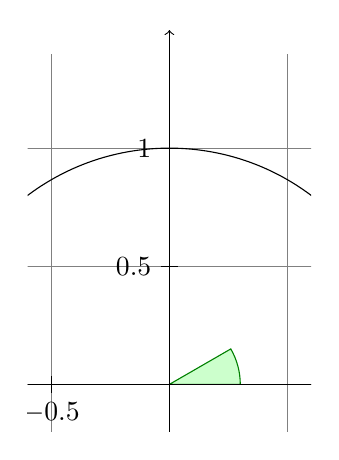
\begin{tikzpicture}[scale=3]
\clip (-0.6,-0.2) rectangle (0.6,1.51);
\draw[step=.5cm,help lines] (-1.4,-1.4) grid (1.4,1.4);
\filldraw[fill=green!20,draw=green!50!black] (0,0) -- (3mm,0mm)
arc [start angle=0, end angle=30, radius=3mm] -- cycle;
\draw[->] (-1.5,0) -- (1.5,0); \draw[->] (0,-1.5) -- (0,1.5);
\draw (0,0) circle [radius=1cm];

\foreach \x in {-1,-0.5,1}
% 在后面那个节点的某个方向添加一个node,名字就是\x变量的名字。
% $\x$就是指获取\x的变量的内涵。
\draw (\x cm,1pt) -- (\x cm,-1pt) node[anchor=north] {$\x$};
\foreach \y in {-1,-0.5,0.5,1}
\draw (1pt,\y cm) -- (-1pt,\y cm) node[anchor=east]  {$\y$};

\end{tikzpicture}


% 这个例子就是在讲/符号的一个简单的用法,无聊。
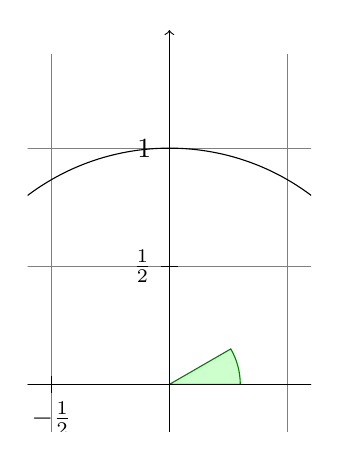
\begin{tikzpicture}[scale=3]
\clip (-0.6,-0.2) rectangle (0.6,1.51);
\draw[step=.5cm,help lines] (-1.4,-1.4) grid (1.4,1.4);
\filldraw[fill=green!20,draw=green!50!black] (0,0) -- (3mm,0mm)
arc [start angle=0, end angle=30, radius=3mm] -- cycle;
\draw[->] (-1.5,0) -- (1.5,0); \draw[->] (0,-1.5) -- (0,1.5);
\draw (0,0) circle [radius=1cm];
\foreach \x/\xtext in {-1, -0.5/-\frac{1}{2}, 1}
\draw (\x cm,1pt) -- (\x cm,-1pt) node[anchor=north] {$\xtext$};
\foreach \y/\ytext in {-1, -0.5/-\frac{1}{2}, 0.5/\frac{1}{2}, 1}
\draw (1pt,\y cm) -- (-1pt,\y cm) node[anchor=east] {$\ytext$};
\end{tikzpicture}

% 下面的例子表面上很复杂,其实只需要在意node可以自定义fill的颜色一点。
\usetikzlibrary {intersections}
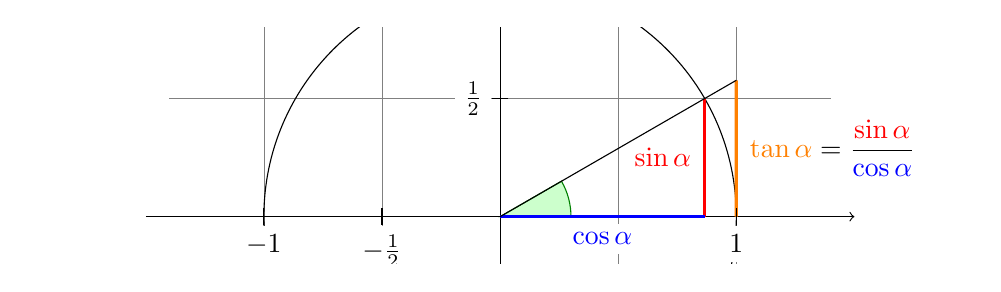
\begin{tikzpicture}[scale=3]
\clip (-2,-0.2) rectangle (2,0.8);
\draw[step=.5cm,gray,very thin] (-1.4,-1.4) grid (1.4,1.4);
\filldraw[fill=green!20,draw=green!50!black] (0,0) -- (3mm,0mm)
arc [start angle=0, end angle=30, radius=3mm] -- cycle;
\draw[->] (-1.5,0) -- (1.5,0) coordinate (x axis);
\draw[->] (0,-1.5) -- (0,1.5) coordinate (y axis);
\draw (0,0) circle [radius=1cm];
\draw[very thick,red]
(30:1cm) -- node[left=1pt,fill=white] {$\sin \alpha$} (30:1cm |- x axis);
\draw[very thick,blue]
(30:1cm |- x axis) -- node[below=2pt,fill=white] {$\cos \alpha$} (0,0);
\path [name path=upward line] (1,0) -- (1,1);
\path [name path=sloped line] (0,0) -- (30:1.5cm);
\draw [name intersections={of=upward line and sloped line, by=t}]
[very thick,orange] (1,0) -- node [right=1pt,fill=white]
{$\displaystyle \tan \alpha \color{black}=
\frac{{\color{red}\sin \alpha}}{\color{blue}\cos \alpha}$} (t);
\draw (0,0) -- (t);
\foreach \x/\xtext in {-1, -0.5/-\frac{1}{2}, 1}
\draw (\x cm,1pt) -- (\x cm,-1pt) node[anchor=north,fill=white] {$\xtext$};
\foreach \y/\ytext in {-1, -0.5/-\frac{1}{2}, 0.5/\frac{1}{2}, 1}
\draw (1pt,\y cm) -- (-1pt,\y cm) node[anchor=east,fill=white] {$\ytext$};
\end{tikzpicture}


% 这个例子是在解释,针对node标记文字形式,你可以采取什么样的形容词
% 里面的词都是字面意思。
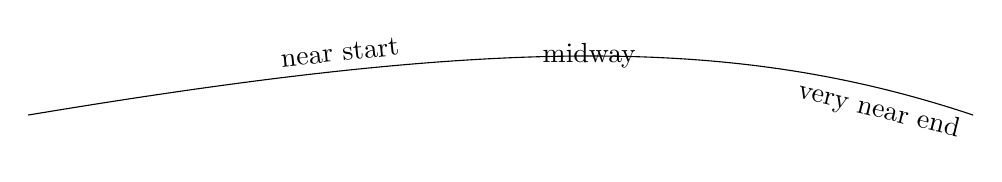
\begin{tikzpicture}
\draw (0,0) .. controls (6,1) and (9,1) ..
node[near start,sloped,above] {near start}
node {midway}
node[very near end,sloped,below] {very near end} (12,0);
\end{tikzpicture}

% 也可以设置长度和高度,这个和latex有点类似。比如:width=6cm


行了,这个东西就这样吧。

\end{document}














%%% Local Variables:
%%% mode: latex
%%% TeX-master: t
%%% End:
